\chapter{Background \& Objectives}
Before commencing the design of the application and the project planning, it is important to have analysed what I hope to have achieved at the end of my project time, and also what steps I will need to be taking to implement each feature. As I will mention later, choosing the best fitting life cycle methodology will play a big part of how I shape my project and create each feature whether it be by priority, size or difficulty. This section details my understanding for my project requirements, steps I am going to need to take, and as I would prefer my project to be similar to and FDD one; developing an overall model and building the list of requirements and features.

\section{Background}
The choice of undertaking a project such as this one was due to two combining factors: maths and an interest to learn graphical programming. The fact that this application will require me to learn graphics, and how to implement visual effects representing the requirements of the project in ways completely new to myself. As graphics is something I have not had much to do with in the past, this project appears both exciting and daunting task due to the learning curve I will need to take. As for the maths factor, I can assume quite a lot of maths will be involved(especially for creating curves, rolls and turns along most of the manoeuvres) which I enjoy learning about.

In terms of the history of the topic, OLAN was originally developed by Michael Gorden in \textbf{2006} and was designed to provide shorthand notation for pilots planning out aerobatic routines without having to draw out the full Aresti diagrams. In recent years, the OLAN notation became used much more until because of licensing issues with the original owner was taken off-line. Because of this, a new form of the notation has been created in a more open source way paving the way for applications such as this project's intended aim. Although in this report and my planned application itself will be still referring the notation as OLAN, the new re-make of the language is known as the \textbf{'OpenAero language'}. This is based off of the original, yet is open and allows anyone to use it. In combination with this, the creators of the OpenAero language also developed a web-based \textbf{application} that allows the conversion of the notations to 2D Aresti diagrams. This is somewhat similar to what I hope to achieve, but alongside plenty more features most importantly the ability to see a plane perform the moves.

As for Aresti, named after its conceiver José Luis Aresti Aguirre \textbf{https://www.aerobatics.org.uk/aresti} is the diagram format that OLAN achieves, and represent informative diagrams showing the shape of the routine, direction of travel, rolls and sharpness of turns. Aresti diagrams also can include angles or turns, ranging from 90 degrees to 270. Each diagram usually has a name, relating normally to the shape of the manoeuvre, though some are more commonly known to pilots rather than the regular user. The OLAN notation for each diagram usually attempts to try describe the manoeuvre with the letter used, such as 'o' for a loop, or 'z' for a shark tooth. The full list of manoeuvres, including their OLAN notation and full name can be found on the \textbf{OpenAero site}.

Upon starting this project, several meetings with the project supervisor are planned each providing more detail of the initial requirements. Each of the meetings will be found in the Gantt for the project, with a smaller document in the\textbf{ appendix} showing the results of each meeting. Because I have already attended several meetings at this stage, I can provide a fairly accurate list of initial requirements of the application.\\

\begin{figure}[h!]
  \centering
      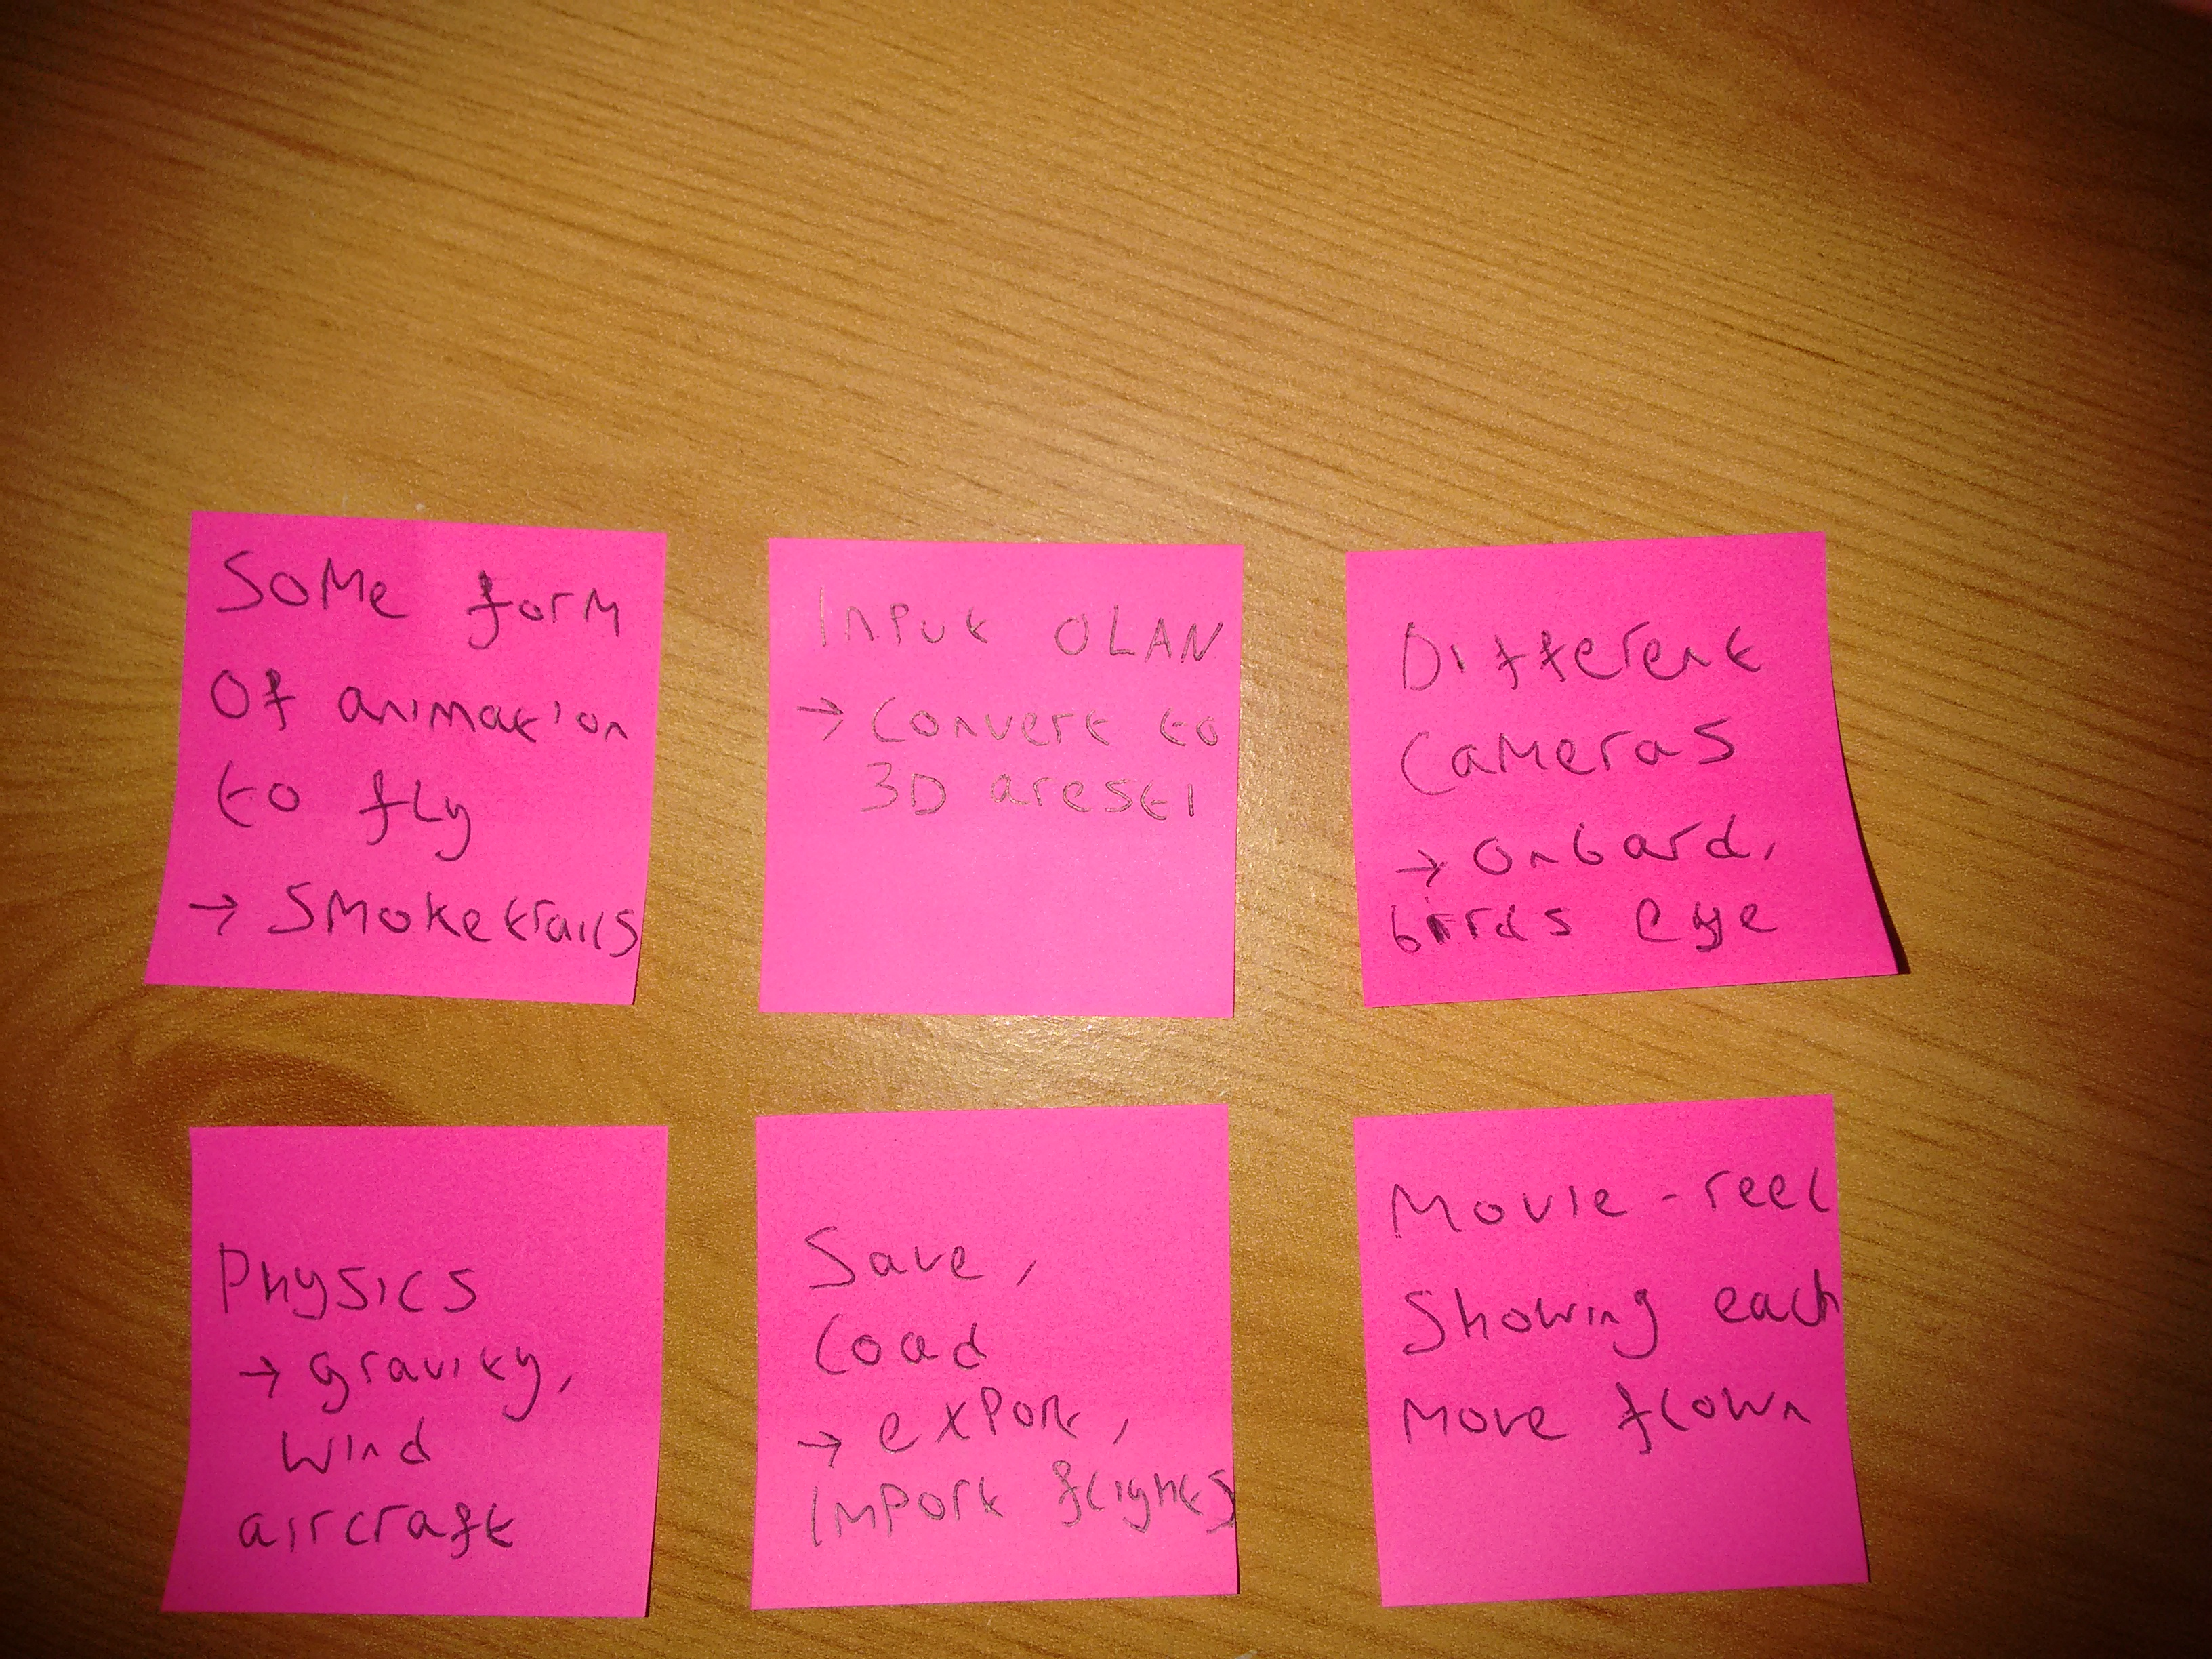
\includegraphics[width=0.5\textwidth]{images/notes.jpg}
  \caption{Image of my initial user stories after my first meeting, short and concise requirements.}
\end{figure}

\noindent The initial required application can be broken down into an extensive(but less detailed) list of main functional requirements. These are as follows:
\begin{enumerate}
	\item Provide a web-implemented tool that allows input of the OLAN 1 None-IE due to WebGL capabilities. Will it use a simple JSON file to store notations? characters as a string format, alongside possible click functionality.
	\item Relate each notation or set of notations to a certain procedural movement(rotations, movements etc.). 
		\begin{itemize}
			\item Must consider parameters in some of the notations, such as the speed of entry.
		\end{itemize}
	\item Provide a means of linking up these movements in such a way into moves, or the angle of the plane. They should produce a fluid manoeuvre.
	\item Display this using WebGL. Libraries to consider that could help. Begin by initially testing simple shapes to move and fly around, then add textures, and plane structure.
	\item Are libraries OK to use? with some of the movements:
		\begin{itemize}
			\item glMatrix- JavaScript library for helping with performing actions to matrices- http://glmatrix.net
			\item ThreeJS- Another JavaScript library, good with handling cameras and different views- http://threejs.org
		\end{itemize}
	\item Allow user to add different effects such as wind, gravity changes and other physics. Could be better to implement these last, as it will be easier to test pure functionality of rolls etc. first, then figure out natural physics.
	\item Add functionalities of different viewpoints(on-board views, side views) to application.
	\item Possibility to add function to save (using local storage?) users different sets of manoeuvres?
\end{enumerate}

The list shown above also has an \textbf{accompanying} report which I created after my first project meeting. This report includes the list of initial requirements, alongside footnotes, and also a detailing of the methodology and process I plan to follow. The document can be found in the appendices section of this report. 

In addition to the list, I feel it should be highlighted why and what language I will be using to create my application. I chose WebGL over OpenGL because of two reasons, the first being that I like the idea of being able to run an application such as this simply in a web browser, without the need for any compilers or platforms installed on the user's device. The other reason being that I already have good experience using JavaScript, and this will help when it comes to the writing code, making sure the coding style is appropriate, and maximising any features it could bring to my application.

\section{Analysis}
Before I begin using my chosen life cycle model, It is important I analyse the overall model and requirements of the intended application. I plan to analyse two items: the requirements analysed by time, effort and difficulty, and also a breakdown of the OLAN and Aresti manoeuvres. The second of which I will break down to their primitive forms, hopefully finding out how I can make my application create each manoeuvre as simple and efficiently as possible.

\subsection{OLAN and Aresti interpretations}
The best place to begin with my analysis is to look in more detail at the OLAN manoeuvres individually, by breaking down each manoeuvre into their primitive elements. As with the previous section, alongside I have attached a document to the appendices of this report, detailing the main and most important manoeuvres I believe are key to finding primitive shapes. I began this by firstly organising each OLAN and their corresponding Aresti shapes into sub groups. 

Of these, there were:
\begin{itemize}
	\item Single element- These include manoeuvres that can be described as one fluid movement. For instance, the OLAN letter 'd' would mean diagonal line up, which requires only one action to complete the manoeuvre.
	\item Two-element- This group includes any manoeuvres that require two separate manoeuvres to complete a given manoeuvres. An example of this could be the 'z' notation, also known as a shark tooth. This shape requires both a diagonal line up followed by a vertical line down. 
	\item Loops- These like the single element moves, consist of a single manoeuvre, and can be combined to make other manoeuvres.
	\item Loop-line combinations- These are loops that are a combination of a loop and a single or two-element manoeuvre.
	\item Double-loops- As the name states, these are manoeuvres that contain two loops.
	\item Humpty-Dumpties, Hammerheads and Tailslides- Each of these manoeuvres represent specific shapes, such as a 'humpty dumpty' which consists of a bump shape comprised of a 180 degree turn to come back down vertically. As the previous, these shapes can simply be combined from single element pieces. 
	\item Complex 3 rolling elements- The naming behind this group of manoeuvres comes from the fact that each contain a set of 3 elements to create the entire figure.
	\item Special and 'oddball' figures- The group of manoeuvres that are more complex in such a way that they require special sections not available from any of the other groups. One example of this is the OLAN letter 'f' which represents a flick. This comprises of rolling the aircraft 360 degrees along its horizontal line.
\end{itemize}

Another important part of the OLAN analysis that I had to understand before proceeding was the possible parameters, prefixes and postfixes that can be attached to manoeuvres. 

Looking at prefixes first, each one-letter-notation, \textbf{some} moves are able to be reversed, or inverted. These are so:
\begin{itemize}
	\item r - Reverse, meaning to order of how each part of the manoeuvre is done. For example, placing the letter 'r' before 'c', would represent a Cuban loop flown in the opposite order. 
	\item i - Inverse, meaning that each part of the manoeuvre is done in the same order, but inverted in terms of value. For example, the letter 'i' before 'c' would mean that rather than looping upwards, the loop would go down. A diagonal line upwards would become a diagonal line downwards.
	\item ir - This is simply a mixture of both the previous. The manoeuvre fixed to the end of this postfix would both be inverted and then reversed. 
\end{itemize}

In addition, there are a number of postfixes that can be used with some manoeuvres particularly with roll or turn based figures. For example, manoeuvres containing rolls can be represented with the prefix angle of turn in multiples of 90 degrees, and a postfix of the amount of rolls along the same part of the path. So in one example, the notation '2j2' would represent a 180 degree turn, whilst rolling the aircraft twice. Alike the prefixes for inverting and reversing manoeuvres, the parameters are not available on all the manoeuvres in the OLAN catalogue. Again, the full list can be found on the the OpenArea site, or see the my OLAN understandings in my \textbf{appendices}.

One final set of optional parameters that could be required of my application to handle are the positions of manoeuvres. Although not strictly in part of the OLAN catalogue, it is already available in the OpenAero application. These parameters are structured (x,y) with x representing the amount of horizontal distance and y the vertical distance from the end of the previous manoeuvre to the start of the current manoeuvre. These can also be negative values to ensure the user can control the position fully. 

The main reason for the need of this is that simply all manoeuvres cannot fully follow each other straight after each other. In real-life if a manoeuvre made the pilot finish near the ground, and the next move required them to perform a diagonal line down, they would hit the ground. Obviously my application will attempt some form of validation and checks, but offering the option to the user is a very useful feature.

From my analysis in the groups listed above, a number of assumptions can be made.
\begin{enumerate}
	\item I have already deduced that all none-single manoeuvres that do not include loops or rolls should be possible to be made from a set of single element manoeuvres.
	\item In total, any manoeuvre can be constructed from one of three primary moves: diagonal and straight lines, curved lines, and turns and rolls. Each of which should be able to carry parameters.
	\item Each curve should be possible to be created based on 45 degree increments, as this is the smallest change of angle in any manoeuvre, and all other angles seem to be in multiples of this number. This will shorten the need for multiple commands for different ranges of angles when programming in the manoeuvres. Because the changes in angle will need to be by a curve, interpolation will be required to make the change in angle smooth and realistic.
	\item Turns, curves and rolls will all need parameters, as some curves are steeper and shorter than others. The same goes for rolls, where you can choose anything from quarter to 3 rolls, and in turns the angle of turn should be specifiable.
\end{enumerate}

By considering my analysis of the set of manoeuvres, I can now envision what manoeuvres will be possible to create easiest, and prioritise my work better. The next section of this report will group up the functionality of the application with my OLAN manoeuvre findings.

\subsection{Application functionality interpretations}
Upon having my initial meetings with the project supervisor, and on analysis of the OLAN catalogue, I can now make more final judgements on what I want to have been achieved by the end of this project. As I discussed in the background section, I had already created a set of initial assumed requirements. Though, some of the features raised questions, such as the possibilities to use libraries for the physics and graphical side. After some research I can now define a more cohesive and stable list of features and requirements of my application. Rather than in a list format though, here I will group features together and discuss the most important factors.

\begin{table}[h]
\caption{A table of prioritised features and tasks that I would like to have implemented by the end of the project. The lower ranked items will only be started on completion of higher tasks.}
 \label{tbl:rank-table}
\begin{tabular}{|l|l|}
\hline
\textbf{Rank} & \textbf{Description}                                                                \\ \hline
1             & Support broken down manoeuvres, via JSON, convert to vectors and ultimately figures \\ \hline
2             & Allow for each manoeuvre to link together, start at end of previous                 \\ \hline
3             & Animate along a path of the manoeuvres                                              \\ \hline
4             & Create cameras, onboard and birds eye                                               \\ \hline
5             & Ground and lighting additions                                                       \\ \hline
6             & Saving and loading of inputs                                                        \\ \hline
7             & Manoeuvre validation                                                                \\ \hline
8             & Physics options, different aircrafts                                                \\ \hline
9             & Movie reel functionality                                                            \\ \hline
10            & Mobile compatibility and nice GUI                                                   \\ \hline
\end{tabular}
\end{table}

Starting with the underlying functionality based on my OLAN interpretations, what I hope to be achievable by the end of this project is the possibility to allow users to enter any length of space separated OLAN characters into an input box, alongside any possible prefixes, postfixes and parameters. I hope to achieve this by making my system as general as possible, and by using very abstract methods that can support any given move input. One way I could think of implementing this now would be to break each manoeuvre into a set of instructions, each one saying which direction to move, the angle and length. By breaking each manoeuvre into these, I could use a single method to construct each manoeuvre on the fly. This is important as it would then allow for the user to play through the manoeuvre in an animated fashion and see the aircraft move.

More generally, one of the questions asked by myself at the start of this project was if libraries could be used to help create the graphics and physics. By now, I have had more meetings with my supervisor and found this was allowable. The main library I have considered after this has been the \textbf{three.js} library which acts as a good wrapper for controlling a wide range of objects in a scene. This library will allow me to easily manipulate vectors, cameras and lighting which will form the basis of my application. I will discuss the use of this library when it comes to planning each of the features in my design.

This brings me to the scene and cameras that I hope to have working to a good standard. For the scene, things such as the ground terrain are not so important, and can simply represent a flat land, while lighting could be added, but perhaps after fundamental features are added. As for cameras, I would like it that there is a set of two cameras: one for navigating and viewing flight paths at different locations and angles, and another camera which would be on-board, like a nose-cam.

The save/ loading of flight paths is a lower ranked task, but something I will definitely be planning to have implemented by the end of the project. Having looked into various methods of saving the OLAN entries, the best way I have found is to use a combination. One which would use local storage, and one that would export to JSON. The first of which I found out \textbf{here} is particularly useful as my project is web based.

There are four features I would also like to add, but I will make these optional for now, and place these after the previously mentioned features. The first of which would be to validate the manoeuvre entry. Currently in the OpenAero application there is a check that looks how close and where manoeuvres are placed on the canvas, and for my application it would be ideal to have a check that looks if manoeuvres are actually possible from the current rotation or placement of the last manoeuvres ending position. Another big check would be if the current path of the aircraft was to hit the floor, a check should be made.

Physics is also an option I would like to include, such as wind, type of aircraft(each aircraft could be more difficult to navigate corners, meaning wider curves). And relating back to the function of playing the animation once the manoeuvres are drawn, an idea passed onto me from my supervisor was of a 'movie-reel' function that would show a mini image of the current manoeuvre being played, showing the animation progressing through each one. Again, this is another feature I would prioritise less, and implement after other key features.

Finally, a more smaller task I think I should set myself is to make the application mobile compatible. As most phones also now have WebGL capabilities, making the application run on mobiles should be possible. This is more a GUI centred feature on the site itself though, and should be added nearer the end of the project.

\section{Process}
Moving onto more project and time management specific items, the process in which I follow can have a large effect on what features I complete on time. At this stage, I would suggest using a hybrid of both the waterfall methodology alongside feature-driven development to create me application. The reasoning for this starts with the way I have already created a list of features in my analysis, which is already part of the FDD life cycle. This would mean following this, I would be able to simply iterate over each feature, plan, implement and test each one by one. This is an ideal trait that comes from using this methodology which allows me to create each feature separately, and more importantly by priority. Then for instance if I was not to finish the entire list I outlined, my application would still have a good deal of functionality on offer. If I were to use the waterfall method alone, It might mean I try implement too many items at once, yet not finish certain parts that rely on others. This would result in an incomplete and less functional program. I feel like there is also a clear part of the scrum methodology put to use here, as I showed with some user stories, and the prioritised list of features.

The second reason, and reason for including the waterfall cycle in my hybrid approach is because I would like to create a more big up front design before beginning implementation. This is where my approach is going to be different from a solely FDD way, where I would usually have to design each feature before implementation and testing. I prefer the way of knowing how the entirety of the structure of code should look before I begin, yet keep the structure as loosely connected as possible to ensure that features avoid relying on each other to an extent where if one is broken, the rest is broken. 

Because I have chosen my methodology in this fashion, has meant I have been able to create a Gantt chart based on stages of planning and design, and also what features I hope to have accomplished at times throughout my project. This, coupled with a work blog, will allow me to track my progress throughout, and compromise when time is needed, or move along the list of features if time is available. I will update my Gantt chart as time progresses in relation to my blog, where I will then be able to see where progress is up to overall.

As for implementation and testing, I will carry out these as normally in the FDD way by implementing and testing each feature one at a time. In the implementation stage of each, I will ensure that decoupling is a priority meaning any developing code does not damage any current working functionality of another feature. The implementation and testing schedules of each feature can be seen on the updated \textbf{Gantt} chart in the appendices. This time, the Gantt chart tasks in to consideration the difficulty and time required to implement and test each feature.